
%%%%%%%%% PROPOSAL -- 15 pages (including Prior NSF Support)


% The research and training plan presents the research that you will conduct and the training 
% that you will receive during the fellowship period and how they relate to your career goals. 
% Include in the research and training plan: 1) a brief and informative introduction or background 
% section; 2) a statement of research objectives, methods, and significance; 3) training objectives 
% and plan for achieving them (these may include scientific as well as other career preparation activities); 
% 4) an explanation of how the fellowship activities will enhance your career development and future 
% research directions as well as describing how this research differs from your dissertation research; 5) 
% a justification of the choice of sponsoring scientist(s) and host institution(s); 6) a timetable with yearly 
% goals with benchmarks for major anticipated outcomes. As with all NSF proposals, broader impacts 
% must also be addressed.
%
% Some applications may require other documentation before the final decision can be made, e.g., 
% animal care and use, human subjects, government permits, letters of collaboration, and commitments 
% from private sources. Their existence should be noted in the research and training plan, but they 
% should not be included in the application. NSF may request them later.

\required{Project Description}

% From the NSF Grants Proposal Guide:
% "The Project Description should provide a clear statement of the work 
% to be undertaken and must include: objectives for the period of the proposed 
% work and expected significance; relation to longer-term goals of the PI's 
% project; and relation to the present state of knowledge in the field, 
% to work in progress by the PI under other support and to work in progress 
% elsewhere."

\begin{wrapfigure}{r}{0.5\textwidth}
\vspace{-30pt}
\centering
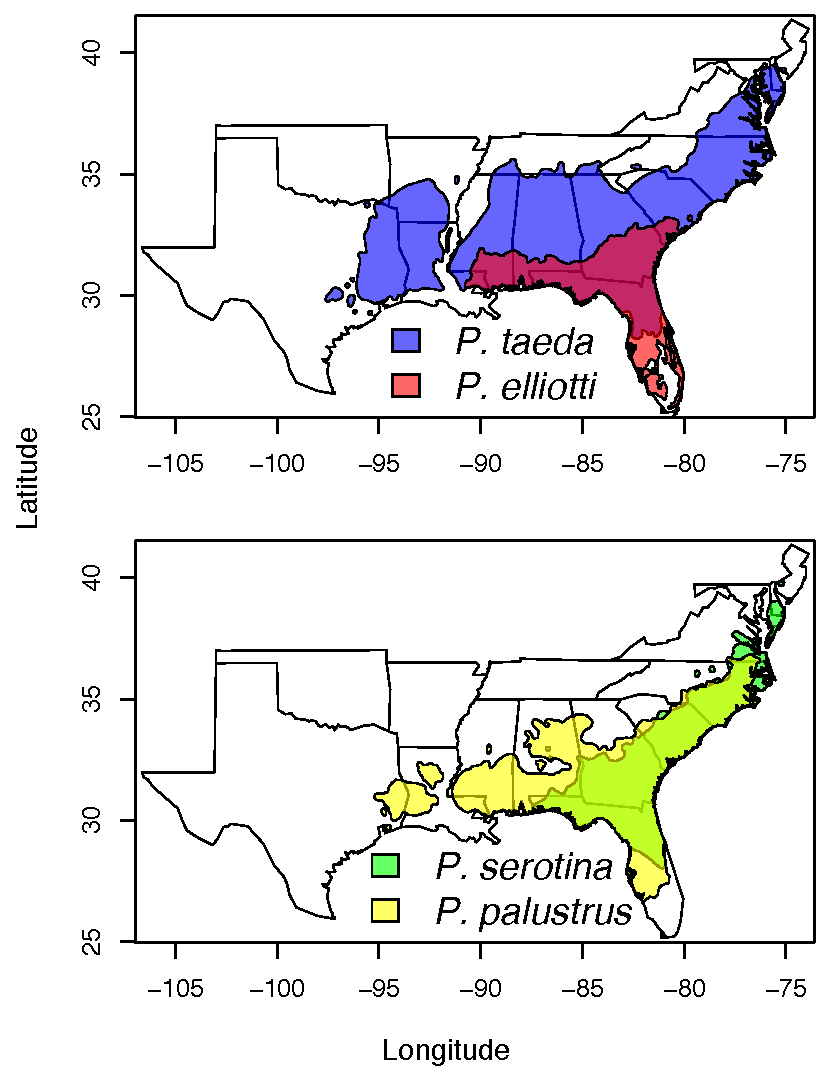
\includegraphics[scale=0.7]{rangemap}
\caption{Natural ranges for four study species}
\label{f:range}
\vspace{-10pt}
\end{wrapfigure}



The PI will investigate local adaptation of a complex trait in 2000 trees from four, economically-important species of pines with a range along 
the eastern and south-eastern United States (25 trees from 20 populations for each specie).  The PI will study 
thick bark (TB), as a quantitative phenotypic trait, in populations of slash pine (\emph{Pinus elliottii}), pond pine (\emph{P.\ serotina}), 
loblolly pine (\emph{P.\ taeda}), and long leaf pine (\emph{P.\ palustris}).  Using next-generation, high-throughput sequencing, the PI 
will dissect TB as a complex adaptive trait across populations of these four closely related species 
with an eye toward uncovering shared genetic architecture at multiple evolutionary times scales.  

Plants display strong patterns of adaptation, especially local adaptation, when populations sizes are large \citep{Leimu:2008fb}.
This characteristic is especially important in conifers, which display a lack of population structure and large effective population 
sizes \citep{Neale:2004hi}; this is partly why association genetic studies have been so successful in these species 
\citep{Eckert:2012cw,Eckert:2010hd, Wegrzyn:2010dd,Eckert:2009hh,GonzalezMartinez:2007gy,GonzalezMartinez:2006ij,Gupta:2005fx}.  
Additionally, because linkage disequilibrium is low in conifer populations, it is possible to detect frequency differences in alleles significantly 
associated with ecologically-relevant phenotypes \citep{Neale:2004hi}. 

Fire has been crucial influence in global ecosystem processes, driving not only locally adapted phenotypes in plant populations 
\citep{Lamont:1991js,Vega:2008vk,Midgley:2011dw,Keeley:2011jw,He:2012bz,Parchman:2012ca}, 
but also impacting carbon storage and climate \citep{Bowman:2009kp}.  Understanding the underlying genetic architecture 
associated with fire-associated traits is therefore critical to dealing with environmental impacts of increased carbon inputs and 
changing climate.  \citet{He:2012bz} recently investigated five fire-adapted traits for 101 species of \emph{Pinus} and found evidence 
for a strong influence of fire in the Cretaceous on trait evolution.  However, they considered only presence or absence the traits in 
their study.  \textbf{There have been no studies to date which capture, as in this proposal, the quantitative nature of fire-associated trait 
evolution in these species.}.  



The application of next-generation sequencing technology to conifer genomes, as proposed in this study, holds the promise of 
being able to provide a way to dissect the genetic architecture of an adaptive, and quantitative trait.  Until recently, techniques 
to consider adaptation on a genomic scale have been no match for the size and complexity of conifer genomes \citep{Mackay:2012hr}.  
\begin{wrapfigure}{r}{0.5\textwidth}
	\begin{ganttchart}[vgrid,
	bar/.style={fill=gray!40}, 
	title/.style={fill=gray!10}]{12}
	\gantttitle{2013}{4}
	\gantttitle{2014}{4}
	\gantttitle{2015}{4}\\
	\ganttbar{Aim 1}{1}{4.5}\\
	\ganttbar{Aim 2}{3.5}{8.5}\\
	\ganttbar{Aim 3}{8.5}{12}
	\end{ganttchart}
\caption{Project timeline}
\vspace{-10pt}
\label{f:timeline}
\end{wrapfigure}
However, advances in genomic enrichment techniques such as those by \citet{Parchman:2012ca} and \citet{Willing:2011jb} and 
the ever-decreasing cost of DNA sequencing have facilitated studies to use genotype-by-sequencing (GBS) approaches to 
answering fundamental questions in evolutionary biology in non-model species.  The PI is well-positioned to utilize the 
sophistication of the sequencing facilities at VCU coupled with his backgrounds in evolutionary, molecular, and 
computational biology to study how thick bark has evolved across \emph{Pinus} and how this knowledge may serve to 
inform ecologically-relevant and economically-important decisions related this important genus.

This study is laid out below in three general aims: (1) field sampling, (2) DNA sequencing and bioinformatics, and (3) 
hypothesis testing.  A projected timeline for this project is shown in Figure \ref{f:timeline}.

\subsection*{Aim 1: Collect field samples, extract genomic DNA, and prepare sequencing libraries}

\paragraph{Field sampling}

The PI will sample four species in their natural ranges, with 25 individuals from 20 natural populations (Figure \ref{f:range}).  
The locations will be determined randomly.  Within each population, a representative 
of the focal species will be chosen and all other members will be chosen from with \SI{50}{m} of the first sampling location meeting 
the requirement of having DBH of at least \SI{15}{\cm}.  Three to five needle fascicles will be collected at each from each 
tree for use in DNA extraction.  Needles, with a desiccant, will be stored in \SI{15}{\ml} Falcon\texttrademark\ tubes  at 
ambient temperatures in the field and in \SI{-80}{\celsius}, long-term in the laboratory.  


Thick bark will be treated as a quantitative character and will be estimated for each tree using a regression model based 
upon tree height and diameter at breast height (DBH) \citep{Cao:1986th, Li:2010bl}.  Measurements of tree height will be obtained using a 
clinometer.  Additionally, measurements of bark thickness will be taken from a representative set of five trees from each population.  
This will allow for the application of a multiple regression model to non-invasively estimate the bark thickness from the other 
\SI{80}{\percent} of the individuals in each population.  Briefly, for each of the sampling trees chosen for invasive sampling, a 
Hagl\"{o}ff\textsuperscript{\textregistered} bark gauge will be used to measure the bark thickness.  These measurements will be used as a covariate in the 
regression equation from \citeauthor{Cao:1986th}, which has been shown to significantly decrease bias by up to \SI{43}{\percent} 
in some species \citep{Li:2010bl}.  At the end of sampling, \num{2000} individual tubes of needles (20--25 needles/tube) 
will be banked along with bark thickness measurements and estimates for all trees for all species.

\paragraph{DNA extraction}
Genomic DNA will be extracted from leaf tissue Qiagen DNEasy extraction kits in a 96-well format using an existing tissue preparation
protocol in the Eckert lab.  A single DNA extraction from multiple leaves per individual will be performed resulting in \num{2000} 
individual genomic DNA extracts.  

\paragraph{Criteria for completion}
Aim 1 will be designated complete when genomic DNA has been extracted for all \num{2000} individuals.  It is estimated that this will be 
complete by June 2014.

\subsection*{Aim 2: Perform sequencing of 2000 individuals and bioinformatic analysis}

The PI will perform genotype-by-sequencing (GBS) utilizing the highly-multiplexed, next-generation sequencing capability of the 
Illumina HiSeq 2000 platform.  Genomic enrichment will be performed using the approach approach outlined in 
\cite{Parchman:2012ca}, in order to ensure high-coverage of the library given the complexity and size of conifer genomes 
\citep{Mackay:2012hr}.  Additionally, each individual will be associated with a computationally-correctable sequencing 
barcode \citep{Roche454MID}.  
Briefly, the genomic DNA from an individual is digested with two different restriction enzymes coupled with Illumina-specific 
adaptor ligation.  The product is amplified by PCR and size selected on an agarose gel, which produces a pool of fragments for 
sequencing.  Estimates for sequencing include approximately 100 individuals per lane on an eight-lane flow cell, with a 
per-lane yield of 200 million reads in a paired-end reaction.  All costs for sequencing will be absorbed by the Eckert lab.  
The result of this aim will be individual FASTQ files, one for each lane in the flow cell containing reads for each multiplexed 
sample in that lane, for each flow cell that is used.  So, if 100 trees are multiplexed per lane, 2.5 flow cells will be needed for 
20 lanes of sequencing.  These 20 lanes will produce four billion reads in total (approximately 8 terabases).  

The Nucleic Acids Research Facility (NARF) at VCU is currently producing paired-end reads of 150 bases, but due to the 
specific error profile of Illumina data, not all of the data is immediately useful.  Using software that the PI has already written 
\citep{code:2008wq} coupled with existing libraries (e.g., BioPython \citep{Cock:2009hj}, NGS QC Toolkit 
\citep{Patel:2012fq}), the processed sequencing data computationally divided into individuals and will be purged of 
low-quality reads. Additionally, reads that meet acceptance criteria globally, but possess bases (most often at the 3' end) 
that have low quality scores, will be trimmed and retained.  The processed sequence data will be stored in both compressed 
FASTA data for distribution via FTP as well as in a relational database to enable both sample tracking and metadata association.

Once quality-controlled reads are obtained for each individual (and each population), they will be aligned (mapped) to the 
most current draft genome of \emph{P. taeda}, available from \url{dendrome.ucdavis.edu}, using the Burroughs-Wheeler aligner 
(BWA) \citep{Li:2009fi}, and SNPs will be called.  Because loblolly pine is in both our experimental sample as well as the source 
of the reference genome, we have a unique opportunity to get a measure of confidence in the read mapping algorithms such as 
BWA as well as in the overall sequencing quality of our data.  A SNP is called at particular alignment positions if there are enough 
high quality reads to indicate a difference between the sample and the reference genome given a model of error. Sequence data 
from NGS technology requires the use of new SNP calling algorithms that properly model all the sources of errors (e.g, base 
calling errors, mapping errors, and sample preparation errors, particularly PCR errors can have a significant impact on the analysis).
Several tools have been developed to perform this task such as as SAMtools \citep{Li:2009ka}, GATK \citep{McKenna:2010bv}, and, 
more recently, GeMS \citep{You:2012iy}.   The result of this aim will be a sample (n = 2000) by SNP matrix (n = thousands) for each 
species (n = 4).  

\paragraph{Criteria for completion} Aim 2 will be complete when all libraries have been sequenced and processed.  Processing 
will include demultiplexing of reads according to individual, quality control processing of the reads, and storage both on disk and 
in a relational database system.  The sequence data will be made available to the scientific community at this point.  Additionally, 
mapping to the loblolly genome and SNP calling will result in a sample by SNP matrix.  This aim is the most computationally 
complex, and should be complete in early summer 2015.  

\subsection*{Aim 3: Perform statistical analysis and hypothesis testing}

\subsubsection*{Question 1: What is the genetic architecture of the thick bark phenotype for the four focal pine species that 
are adapted to fire?}

\paragraph{Null hypothesis} $H_0$: There is no association between genotypic variation at surveyed SNPs and thick bark 
phenotypes in any of the four species.

\paragraph{Methods} The PI will employ standard linear models that correct for kinship and population structure that are 
commonly used in genome-wide association studies (GWAS; \citet{Yu:2006ij}). Association analysis has been widely 
used in and has for dissecting the genetic basis of phenotypes for conifers \citep{Neale:2011jh, Ingvarsson:2011fg}. 
In addition, the PI will explore the use of the Bayesian models presented by \citet{Parchman:2012ca}, which 
was the first GWAS for a conifer, and regression tree approaches presented by \citet{Holliday:2012fz}. 
Linear models will be used to explicitly test the effects of genotypic class of each discovered SNP on quantitative 
measures of bark thickness for each species. Thus, the number of tests for genotypic effects for each species will 
be equal to the number of discovered SNPs, which is expected to be in the range of \num{50000} to \num{100000}. 
\citet{Parchman:2012ca}. Multiple tests will be accounted for using a permutation approach that adjusts the 
global significance level (e.g., $\alpha= 0.05$). In brief, this procedure randomizes genotypic vectors relative to the 
phenotypic vector to produce a large number of randomized data sets (e.g. \num{10000}). For each randomized data 
set, the association analysis is conducted again and the minimum \emph{P}-value associated with a genotypic effect is 
retained. Finally, the multiple-test corrected $\alpha = 0.05$ is then the \SI{5}{\percent} quantile of the distribution of 
minimum \emph{P}-value. 

\paragraph{Expected outcomes and relevance} The null hypothesis will be rejected when at least one SNP in each 
of the four pine species is significantly associated to quantitative variation in bark thickness. Previous association 
studies in conifers typically identify five to 20 plus SNPs associated with the trait under consideration 
\citet{Eckert:2012cw}. These results will classify SNPs discovered into each species into two classes: those 
associated to bark thickness (which rejects the null hypothesis for this question) and those unassociated with 
bark thickness. The latter will be used as controls for questions two through four. The former establishes the 
genetic architecture of bark thickness for each focal species.

\subsubsection*{Question 2: Is the identified genetic architecture (e.g. the set of SNPs for each species) from Question 1 
shared across the four focal species, and if so, is it shared to a greater extent than random variation within the 
genomes of these four closely related species?}

\paragraph{Null hypotheses}  ${H_{0}}^1$: There is no shared genetic architecture for bark thickness among 
the four focal species. ${H_{0}}^2$: The degree of allele sharing is greater for loci associated to 
bark thickness than randomly selected loci.

\paragraph{Methods} To evaluate ${H_{0}}^1$, the PI will leverage the underlying, queryable data storage infrastructure 
to produce the intersection of SNPs associated with bark thickness in all four focal species.  From Aim 2, confidence in SNP 
calls can be quantified because the genome of the reference organism is represented in the set of focal species.  
To evaluate ${H_{0}}^2$, the union of all SNPs associated with bark thickness 
will be created. The fraction of this list that is shared across all four species will be used as a test statistic, the magnitude 
of which will be tested via a simple permutation analysis. The PI will construct a null distribution for the fraction of alleles 
shared across all four species for sets of SNPs randomly selected from those unassociated to bark thickness (see Question 1). 

Allele sharing across species is common among conifer species and has been attributed largely to incomplete lineage 
sorting resulting from recent divergence times and large effective population sizes \citep{Syring:2007gd,Willyard:2009ez}, 
ancient admixture \citep{Liston:2007cx} and 
long-term gene flow \citep{Zhou:2010hk}. For example, an analysis of 
levels of long-term gene flow between loblolly and slash pines using multiple random sets of 50 nuclear genes and an 
isolation-with-migration model \citep{Becquet:2007js} detected low but significant levels of gene flow over the divergence history 
of these species (unpublished data, $4 N_{e}m = 2.5$ with a \SI{95}{\percent} confidence interval of 0.52--5.14). The sets of loci 
randomly sampled from the unassociated loci will be assumed to largely reflect these processes, so that the 
enrichment of allele sharing at loci associated to a trait such as bark thickness with clear adaptive relevance 
\citep{He:2012bz} would imply additional processes such as natural selection, as in \cite{Segurel:vf}, in promoting allele 
sharing among species.

\paragraph{Expected outcomes and relevance} ${H_{0}}^1$ will be rejected when multiple SNPs (i.e., $> 5$) associated 
with bark thickness are shared across species. The relevance of this result would be to establish the shared genetic 
architecture of an adaptive trait. ${H_{0}}^2$ will be rejected when the fraction of SNPs associated to bark thickness that are 
shared across the four focal species lies in the upper \SI{1}{\percent} tail (i.e., $\alpha = 0.01$ for a one-tailed test) 
of the null distribution based upon random sets of unassociated SNPs. The relevance of this result would be to 
establish that a process beyond incomplete lineage sorting, admixture and gene flow is contributing to the 
maintenance of trans-species 
polymorphisms across the four focal species. 


\subsubsection*{Question 3: Are reconstructed allele frequencies at shared SNPs that are associated with bark thickness 
correlated more so with reconstructed bark thickness than randomly selected shared SNPs that are unassociated with bark 
thickness across the phylogeny for these four species?}

\paragraph{Null hypothesis} $H_0$: Correlations between reconstructed allele frequencies at shared SNPs associated with 
bark thickness and reconstructed values of bark thickness are no larger than those for reconstructed allele frequencies at 
randomly chosen SNPs unassociated with bark thickness.

\paragraph{Methods} Phylogenies and associated data matrices for genus \emph{Pinus} will be obtained from 
TreeBASE and GenBank. Most data matrices are constructed primarily from cpDNA coding sequences 
(e.g. Eckert and Hall 2006; Gernandt et al. 2008) and cpDNA genome sequences (e.g. Parks et al., 2008). 
Chronograms will be obtained using the fossil calibration points from Willyard et al. (2008). 
{Chris: insert some language about how the final tree will be constructed [supertree, supermatrix] 
or are we just using the one from He et al. 2012?} Once a set of plausible chronograms has been 
generated, bark thickness and allele frequencies within lineages will be reconstructed as quantitative 
characters using a Bayesian method (i.e. BayesTraits, see Pagel 1997, 1999). 
Specifically, we will utilize a set of plausible chronograms (n =  10,000) to account for uncertainty in 
phylogenetic tree and the character states in combination with phylogenetically informed multiple 
regression analyses (available in BayesTraits as BayesContinuous) to test the association with 
reconstructed SNP allele frequencies and bark thickness for two types of SNPs: those shared across 
all four species and associated with bark thickness versus those shared across all four species and 
unassociated with bark thickness. Allele frequencies and bark thickness will be specified for each species 
as averages and variances across populations.

\paragraph{Expected outcomes and relevance} $H_0$ will be rejected when the multiple regression model for the 
SNPs associated with bark thickness better predicts bark thickness than those for SNPs unassociated with bark thickness. 
This suggests that the correlation structure of allele frequencies with bark thickness differs between the candidates and controls 
as defined by answering questions 1 and 2. Since controls are matched in number and levels of heterozygosity with the candidates, 
this would suggest non-neutral processes driving this difference.

\subsubsection*{Question 4: To what extent is natural selection maintaining the fire-associated, thick bark phenotype in these focal species?}

\paragraph{Null hypothesis} $H_0$: There is no evidence of selection in genes containing SNPs that are significantly associated 
with thick bark.

\paragraph{Methods} As the loblolly pine genome continue to improve, establishing the genomic context of thick 
bark-associated SNPs will enable the PI to test for evidence of selection in polymorphic, protein coding genes.  The PI will select 
10 to 20 SNPs from a subset of associated loci from each population for each species.   Using genomic position of SNPs and the loblolly 
genome annotations, the PI will design PCR primers to amplify the protein coding regions from each tree, and each amplicon will be sent 
for Sanger sequencing.  Once the sequences have been obtained and translated to amino acids, they will be aligned at the amino acid level 
using standard tools such as MAFFT \citep{Katoh:2005ia} or MUSCLE \citep{Edgar:2004ic}.  From the alignment (back-translated to DNA), 
$d_N/d_S$ will be estimated using established maximum likelihood methods \citep{Yang:2007ki}.

\paragraph{Expected outcome and relevance}  Knowing whether or not genes containing SNPs are under positive ($d_N/d_S > 1$) or 
purifying selection ($d_N/d_S < 1$) addresses a fundamental question surrounding maintenance of these polymorphisms in 
natural populations.  

\required{Broader Impacts}
% as in the project summary, broader impacts must be called out separately 
% in the project description.  You may be able to give more specific
% examples, or discuss how you've previously achieved these impacts.
% It should be similar, but not identical, to the Broader Impacts statement
% in the project summary
This project will benefit both the local and global scientific communities, as well as help train 
the next generation of multi-discipline scientists in the world of big data.  First, as soon as the data is curated, it will be made 
available for download and exploration from FTP and web sites hosted here at VCU.  Second, the PI will develop and teach a new 
three-credit course, BIOL 591 Applied Ecological Genomics, which will train advanced undergraduates and established 
graduate students, using the data generated in this project, in skills necessary to both understand the 
technology available at VCU (e.g., Illumina HiSeq/MiSeq, 454, IonTorrent), and to 
process (via programming), manage (via databases), and analyze the deluge of data generated from current genomics 
projects.  This course will run in conjunction with an existing course, BIOL 693 Ecological Genomics taught by sponsor Eckert, 
and has received approval from the Biology department chair.

Given the diverse student body at VCU, the proposed research and 
teaching activities will increase research opportunities for underrepresented groups. VCU is among the top 20 universities in the 
nation for Biology degrees awarded to ethnic and racial minority students. In 2009, 18.3\% of baccalaureate Biology degrees were 
conferred to African American students, exceeding the national average in Biology by 11.5\% (NSF, 2010). A high percentage of 
VCU Biology (39.4\%) baccalaureate degrees were also earned by Asian/Pacific Islanders, a value that far exceeds the 
national average in Biology of 6.2\%. Caucasian students were awarded 34.9\% of VCU baccalaureate Biology degrees as 
compared with the national average in Biology of 66.4\% (NSF, 2010).

\required{Results From Prior NSF Support}
% 5 pages or fewer of the 15 pages for entire description document.
% include results from NSF grants received in the past 5 years.
% if supported by more than one grant, choose the most relevant one
% for each grant, include: NSF award number, amount, dates of
% support, and publications resulting from this research.
% due to space limitations, it is often advisable to use citations rather
% than putting the titles of the publications in the body 
% of this section

% e.g.: "My prior grant, "Uses of Coffee in Mathematical Research" (DMS-0123456, 
% $100,000, 2005-2008), resulted in 3 papers [1],[2],[3], demonstrating..."

% if requesting postdoctoral research salary, a supplemental 1-page document
% called "Postdoc Mentoring Plan" will be required 

PI Friedline has yet to receive funding from the National Science Foundation.